\subsection{The Disordered Ising Model}
\label{ssec:isingmodel}
    The examined model is a modified 2D Ising model.
    First, let's define the Ising model and then explain the modifications.
    The Ising model is a square lattice with edge length \(L\) and
    \(N=L^2\) sites. Each site has a magnetic moment, the spin. Each
    spin can take a value \(s \in \{-1,+1\}\) and interacts with it's
    nearest neighbors described by the hamiltonian from eq. \eqref{eq:hamiltonian}
    \begin{equation}
        \hat{H} = \sum_{\avg{i,j}}J_{ij}s_{i}s_{j} - H \sum_i s_i
        \label{eq:hamiltonian}
    \end{equation}
    \(\avg{i,j}\) refers to nodes \(i\) and \(j\) which are nearest
    neighbors. And \(J_{ij}\) is the coupling constant between \(i\) and
    \(j\). Let the magnetic field \(H=0\).\\
    In this thesis the sites of the square lattice are displaced. The
    displacement is randomly gauss distributed with the standard
    deviation \(\sigma\). This \(\sigma\) is also called
    \emph{disorder paramter} in the following.
    To determine nearest neighbors, edges are constructed according to
    one of the two the in section \ref{ssec:graphtypes} defined rules.
    So that the lattice represents a proximity graph. Each node \(i\)
    has a spin \(s_i = \pm 1\). Each edge \(E_{ij}\) has a weight
    \(J_{ij} = \exp (\alpha (1-d_{ij}))\). \(d_{ij}\) is the Euclidian
    distance between the nodes \(i\) and \(j\) and \(\alpha = 0.5\).
    \(J\) is called \emph{coupling constant}. This is definition is
    inspired by \cite{Lima2000}.\\
    For \(\sigma = 0\) this is the standard Ising model with \(J = 1\),
    for which exists an analytical solution \cite{Onsager1944}.\\

\subsection{Gabriel- and Relative Neighborhood Graph}
\label{ssec:graphtypes}
    A graph \(G(V,E)\) is a set of nodes \(V\) and edges \(E\).\\
    All here mentioned graph types are \emph{proximity graphs}. They are
    connecting nodes which are by some metric near to each other.
    Hence they are suited to generalize problems defined on regular
    lattices with nearest neighbor relationships, like the Ising model
    which will be described in more detail in section
    \ref{ssec:isingmodel}.
    In this thesis the distance is always determined by the Euclidian
    metric in two dimensions, though in principle every metric in any
    dimension can be used.\\

    The Gabriel graph \cite{Gabriel1969} is a subgraph of the
    Delaunay triangulation. Two nodes \(i\) and \(j\) with distance
    \(d_{ij}\) are connected with an edge, if a circle with it's
    center on the middlepoint between \(i\) and \(j\) and radius
    \(r = \frac d 2\) contains no other nodes. This area will be
    called \emph{lune} in the following. See also Figure
    \ref{fig:lunes}\subref{sfig:lunes:def}.\\
    The Relative Neighborhood graph \cite{Toussaint1980} is a
    subgraph of the Gabriel graph. Two nodes \(i\) and \(j\) with
    distance \(d_{ij}\) are connected, if no other node is in the
    \emph{lune}. The lune is defined as the intersection of two
    circles with radius \(r = d\) and centers on \(i\) and \(j\).
    See also Figure \ref{fig:lunes}\subref{sfig:lunes:def}.
    \begin{figure}[htbp]
        \centering
        \subfigure[Definition of the lunes][]{
            \label{sfig:lunes:def}
            \tikzset{
    hatch distance/.store in=\hatchdistance,
    hatch distance=10pt,
    hatch thickness/.store in=\hatchthickness,
    hatch thickness=2pt
}

\makeatletter
\pgfdeclarepatternformonly[\hatchdistance,\hatchthickness]{flexible hatch no}
{\pgfqpoint{0pt}{0pt}}
{\pgfqpoint{\hatchdistance}{\hatchdistance}}
{\pgfpoint{\hatchdistance-1pt}{\hatchdistance-1pt}}%
{
    \pgfsetcolor{\tikz@pattern@color}
    \pgfsetlinewidth{\hatchthickness}
    \pgfpathmoveto{\pgfqpoint{0pt}{0pt}}
    \pgfpathlineto{\pgfqpoint{\hatchdistance}{\hatchdistance}}
    \pgfusepath{stroke}
}
\makeatletter
\pgfdeclarepatternformonly[\hatchdistance,\hatchthickness]{flexible hatch nw}
{\pgfqpoint{0pt}{0pt}}
{\pgfqpoint{\hatchdistance}{\hatchdistance}}
{\pgfpoint{\hatchdistance-1pt}{\hatchdistance-1pt}}%
{
    \pgfsetcolor{\tikz@pattern@color}
    \pgfsetlinewidth{\hatchthickness}
    \pgfpathmoveto{\pgfqpoint{0pt}{\hatchdistance}}
    \pgfpathlineto{\pgfqpoint{\hatchdistance}{0pt}}
    \pgfusepath{stroke}
}

\begin{tikzpicture}
    \clip (-2,2.25) rectangle (2,-1.75);

    \begin{scope}
        \clip (-1, 0.5) circle(2.06155281281);
        %~ \fill[fill=blue!20] (1, 0) circle(2.06155281281);
        %~ \draw[pattern=north west lines] (1, 0) circle(2.06155281281);
        \draw[pattern=flexible hatch no,hatch distance=10pt,hatch thickness=0.7pt] (1, 0) circle(2.06155281281);
    \end{scope}

    %~ \fill[fill=white] (0, 0.25) circle(1.0307764064);
    %~ \draw[pattern=north east lines] (0, 0.25) circle(1.0307764064);
    \draw[pattern=flexible hatch nw,hatch distance=10pt,hatch thickness=0.7pt] (0, 0.25) circle(1.0307764064);
    \draw[thick] (0, 0.25) circle(1.0307764064);

    \draw[thick] (-1, 0.5) circle(2.06155281281);
    \fill (-1, 0.5) circle(0.1);
    \draw[thick] (1, 0) circle(2.06155281281);
    \fill (1, 0) circle(0.1);
    \draw[thick] (1, 0) -- (-1, 0.5);
\end{tikzpicture}

        }
        \subfigure[Relative Neighborhood graph example][]{
            \label{sfig:lunes:rng}
            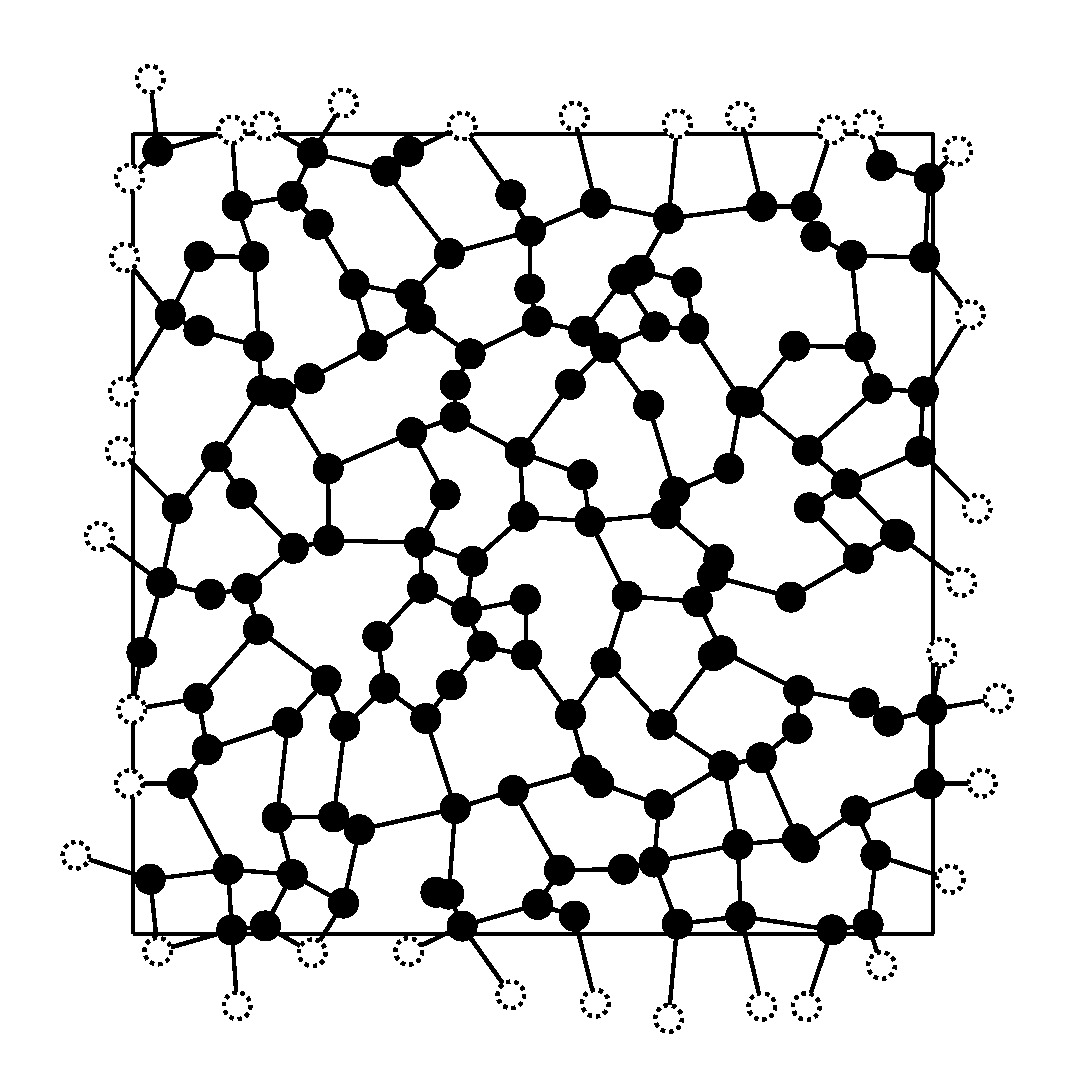
\includegraphics[width=0.3\textwidth]{images/RNG/L12S03.pdf}
        }
        \subfigure[Gabriel graph example][]{
            \label{sfig:lunes:gg}
            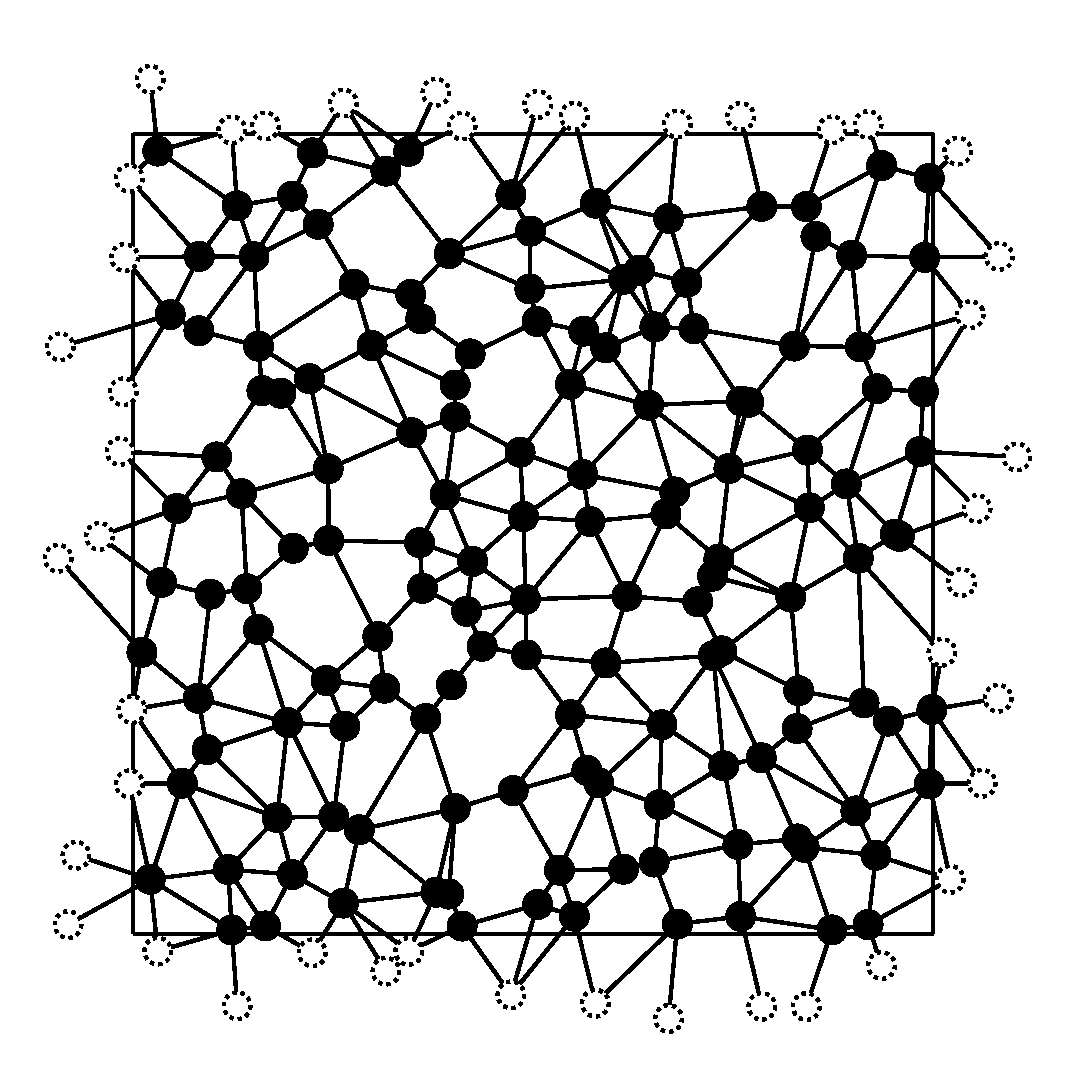
\includegraphics[width=0.3\textwidth]{images/GG/L12S03.pdf}
        }
        \caption[Gabriel - and Relative Neighborhood Graph]
        {
            \subref{sfig:lunes:def} Lunes of Relative Neighborhood
                Graph (hatched region) and
                Gabriel Graph (cross hatched region)
            \subref{sfig:lunes:rng} Example of a Relative
                Neighborhood Graph on periodic boundary conditions.
                Periodic nodes are dashed.
            \subref{sfig:lunes:gg} Example of a Gabriel Graph on
                periodic boundary conditions. Periodic nodes are
                dashed.
        }
        \label{fig:lunes}
    \end{figure}\\
    To construct these graphs the simple way is to test for each
    pair of nodes one has to check for every other node if it lies in
    the lune of the pair. That is of complexity \(O (N^3)\), because
    there are \(N(N-1)\) pairs and for each \(N-2\) nodes to test. So
    the product is of order \(O(N^3)\)\\
    To reduce the complexity one can first create a Delaunay
    Triangulation in complexity \(O (N \log N)\)
    \cite{Leach1992} and test the criterion for each edge, because
    the Delaunay triangulation is a supergraph of both. But the
    implementation of a Delaunay triangulation algorithm is not trivial
    and the generation of the graphs is not time critical in the scope
    of this bachelor thesis.\\
    So a tradeoff is to use basicly the simple method but only test
    the criterion for nodes which are near to the lune and abort if
    one node inside the lune is found. To determine which nodes are
    near the lune one can subdivide the area in \emph{cells} and save
    for each cell a list with nodes lying inside it like presented in
    \cite{RNGCell}.
    Now it is just neccessary to test the nodes in the cells which
    resemble a rectangular bounding box of the lune. Most pairs will be
    far away from each other and the cells in the middle of the bounding
    box are completely inside the lune so that only one node has to be
    tested to discard an edge between them. Connected nodes are near to
    each other so that only very few cells have to be tested.\\
    Indeed this method reduced the time needed to construct a Relative
    Neighborhood graph with \(N=32^2\) and \(N=64^2\) by a factor of
    over \(15\) respectivly \(40\). Though the complexity is still of
    order \(O(N^2)\) in the best case, because for every pair at least
    one check has to be performed.
